%%%%%%%%%%%%%%%%%%%%%%%%%%%%%%%%%%%%%%%%%
%
% (c) 2021 by Jennifer Laaser
%
% This work is licensed under the Creative Commons Attribution-NonCommercial-ShareAlike 4.0 International License. To view a copy of this license, visit http://creativecommons.org/licenses/by-nc-sa/4.0/ or send a letter to Creative Commons, PO Box 1866, Mountain View, CA 94042, USA.
%
% The current source for these materials is accessible on Github: https://github.com/jlaaser/pogil-polymers
%
%%%%%%%%%%%%%%%%%%%%%%%%%%%%%%%%%%%%%%%%%

\renewcommand{\figpath}{content/polymchem/freeradical/FRPthermo/figs}
\renewcommand{\labelbase}{FRPthermo}

\begin{activity}{Thermodynamics of Free-Radical Polymerization}

\begin{instructornotes}
	This activity introduces students to concepts related to the thermodynamics of free-radical polymerization.
	
	After completing this activity, students will be able to:
	\begin{enumerate}
		\item ...
	\end{enumerate}
	
	\subsection*{Activity summary:}
	\begin{itemize}
		\item \textbf{Activity type:} Learning Cycle
		\item \textbf{Content goals:} Thermodynamics of free-radical polymerization
		\item \textbf{Process goals:} %https://pogil.org/uploads/attachments/cj54b5yts006cklx4hh758htf-process-skills-official-pogil-list-2015-original.pdf
			written communication, critical thinking, information processing
		\item \textbf{Duration:} TBD
		\item \textbf{Instructor preparation required:} none beyond knowledge of relevant content
		\item \textbf{Related textbook chapters:}
			\begin{itemize}
				\item \emph{Polymer Chemistry} (Hiemenz \& Lodge): section NNN
			\end{itemize}
		%\item \textbf{Facilitation notes:}
		%	\begin{itemize}
		%		\item \dots
		%	\end{itemize}
	\end{itemize}
	
\end{instructornotes}


\begin{model}[Thermodynamics of Propagation]
	\label{\labelbase:mdl:propthermo}

	The propagation step of a free-radical polymerization is shown below:
	
	\centerline{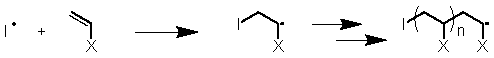
\includegraphics[width=0.8\textwidth]{\figpath/Model1-prop}}
	
	%In this model, we will investigate the thermodynamics of this propagation step.
	
\end{model}


\begin{ctqs}

	\question First, let's think about the enthalpy of the radical center. \label{\labelbase:ctq:radicalenthalpy}
	
		\begin{enumerate}
		
			\item Does the ``type'' of radical change in this propagation step?
				
				\begin{solution}[0.5in]
				\end{solution}
			
			\item Based on your answer to part (a), do you expect the radical center to contribute significantly to the enthalpy of the reaction?  Briefly explain your group's reasoning.
				
				\begin{solution}[1in]
				\end{solution}
			
		\end{enumerate}
		
	\question Second, let's think about the enthalpy of the bonds. \label{\labelbase:ctq:bondenthalpy}
	
		\begin{enumerate}
			\item How does the number of C-C single bonds change in this propagation step?
				
				\begin{solution}[1in]
				\end{solution}
			
			\item How does the number of C=C double bonds change in this propagation step?
				
				\begin{solution}[1in]
				\end{solution}
			
			\item Typical enthalpies for C-C and C=C bonds are summarized below:
				
				\begin{center}
					\renewcommand{\arraystretch}{1.5}
					\begin{tabular}{c c}
						\hline
						Bond Type & $\Delta H$ (kJ/mol) \\\hline
						C-C	&	-350 \\
						C=C &	-610 \\\hline
					\end{tabular}
				\end{center}
				
				Based on this information, calculate the enthalpy change in the propagation reaction shown in Model \ref{\labelbase:mdl:propthermo}.
				
				\begin{solution}[1.25in]
				\end{solution}
		\end{enumerate}
		
	\question Based on your answers to CTQs \ref{\labelbase:ctq:radicalenthalpy} and \ref{\labelbase:ctq:bondenthalpy}, do you expect the propagation step to be exothermic (releases heat) or endothermic (requires heat input)?
	
		\emph{Hint: remember that negative values of $\Delta H$ correspond to exothermic reactions.}
				
				\begin{solution}[0.75in]
				\end{solution}
		
	\question Next, let's consider how the entropy changes in this propagation step.
	
		\begin{enumerate}
			
			\item How does the total number of molecules present in the reaction mixture change in this reaction?
				
				\begin{solution}[0.5in]
				\end{solution}
			
			\item Does the translational freedom of the monomer increase or decrease as it attaches to the polymer chain?
				
				\begin{solution}[0.5in]
				\end{solution}
			
			\item Based on your answers to the previous two questions, do you expect the overall entropy of the system to increase or decrease in this propagation step?  Briefly explain your group's reasoning.
				
				\begin{solution}[1.5in]
				\end{solution}
			
		\end{enumerate}
	
	\question Based on your answers, would you characterize the propagation step in free-radical polymerization as an ``enthalpy-driven'' reaction or as an ``entropy-driven'' reaction?  Briefly explain your group's reasoning.
	
		\begin{solution}[1.5in]
		\end{solution}

\end{ctqs}




\begin{model}[Equilibrium of Propagation]
	\label{\labelbase:mdl:propequilib}

	In our discussion of the kinetics of free radical polymerization, we depicted propagation as being a ``one-way street'' - i.e. the reaction arrow only pointed to the right:
	
	\begin{equation*}
		\text{\ce{P_n^.} + M} \xlongrightarrow{} \text{\ce{P_{n+1}^.}}
	\end{equation*}
	
	However, in reality, this reaction can actually go either forward or backward, and it is more appropriate to write it as an equilibrium, as follows:
	
	\begin{equation*}
		\text{\ce{P_n^.} + M} \rightleftharpoons{} \text{\ce{P_{n+1}^.}}
	\end{equation*}
	
	At equilibrium, the concentration of monomer in the reaction mixture will be $[\text{M}]_{eq}$.
	
\end{model}


\begin{ctqs}

	\question Write an appropriate equilibrium constant for this reaction, in terms of [\ce{P_n^.}], [\ce{P_{n+1}^.}], and $[\text{M}]_{eq}$.
				
				\begin{solution}[1in]
				\end{solution}
	
	\question In most polymerizations, [\ce{P_n^.}]$\approx$[\ce{P_{n+1}^.}].  Use this approximation to rewrite your equilibrium constant from the previous problem as a function of the equilibrium momonomer concetration, $[M]_{eq}$, only.
				
				\begin{solution}[1in]
				\end{solution}
	
	\question Recall that a reaction is in equilibrium when $K = e^{-\Delta G^\circ/RT}$.  Use this relationship, and the fact that $\Delta G = \Delta H - T\Delta S$, to write an appropriate expression relating the equilibrium monomer concentration to the $\Delta H$ and $\Delta S$ of the propagation reaction.
				
				\begin{solution}[1.5in]
				\end{solution}
	
	\question Solve for the temperature, $T_c$, at which the reaction is in equilibrium with a monomer concentration $[\text{M}]_{eq}$.
				
				\begin{solution}[2in]
				\end{solution}
	
	\question Suppose you have a polymerization reaction whose equilibrium monomer concentration is $[M]_{eq}$.  
		\begin{enumerate}
			\item If you start a reaction with a concentration of monomer $[\text{M}] < [\text{M}]_{eq}$, will any polymer form?  Why or why not?
				
				\begin{solution}[1.25in]
				\end{solution}
				
			\item If you start a reaction with a concentration of monomer $[\text{M}] > [\text{M}]_{eq}$, will any polymer form?  Why or why not?
				
				\begin{solution}[1.25in]
				\end{solution}
				
			\item Once a polymerization reaction consumes enough monomer to reach its equilibrium monomer concentration, will the polymer chains continue to grow?  Explain your group's reasoning in 1-2 complete sentences.
				
				\begin{solution}[1.5in]
				\end{solution}
				
		\end{enumerate}

	\question Explain why $T_c$ (which we refer to as the ``ceiling temperature'' of the reaction) can be considered to be the maximum temperature at which polymer will form.
				
				\begin{solution}[1.5in]
				\end{solution}

\end{ctqs}



\begin{model}[Changes to Reaction Rates During Polymerization]
\label{\labelbase:mdl:rxnrates}

	In our derivation of the kinetics of free radical polymerization, we assumed that the rate constants for each step ($k_d$, $k_p$, and $k_t$) did not change over the course of the reaction.  In real polymerizations, however, this does not always hold true.

\end{model}

\begin{ctqs}

	\question As a polymerization reaction progresses, and more and more and more monomer is converted to polymer, what do you expect to happen to the viscosity of the reaction mixture?  Explain your group's reasoning in 1-2 complete sentences.
	
		\begin{solution}[2in]
		\end{solution}
		
	\question As the viscosity of the reaction mixture changes, do you expect it wil become easier or harder for two propagating radicals to find each other and undergo a termination reaction?  Explain your group's reasoning in 1-2 complete sentences.
	
		\begin{solution}[1.5in]
		\end{solution}
	
	\question Based on your group's answers to the preceding two questions, how do you expect the termination rate to change as the reaction progresses?
	
		\begin{solution}[1in]
		\end{solution}
	
	\question Recall that the overall propagation rate in a free-radical polymerization is given by
					\begin{align*}
						R_p = k_p\text{[M]}\left(\frac{fk_d[Init]}{k_t}\right)^{1/2}
					\end{align*}
		Based on this equation, and your answer to the previous question, how do you expect the overall propagation rate to change as the reaction progresses?
	
		\begin{solution}[1in]
		\end{solution}
		
	\question Finally, since propagation is exothermic, what do you expect to happen to the temperature of the reaction mixture as the reaction progresses?  Explain your group's reasoning in 1-2 complete sentences.
	
		\begin{solution}[2in]
		\end{solution}
		
\end{ctqs}

	\begin{infobox}
		The process you have just explored is the \emph{autoacceleration} of free-radical polymerizations.  This effect is sometimes also called the \emph{Trommsdorff Effect}.
		
		Autoacceleration can lead to significant safety problems, including explosions of storage tanks and/or reactor vessels as the temperature increase causes monomers to rapidly vaporize and exceed the pressure capacities of the vessels.
		
	\end{infobox}


\begin{ctqs}

	\question Suggest at least one way that the reaction conditions for a free-radical polymerization could be adjusted to minimize the risk of autoacceleration.
	
		\begin{solution}[2in]
		\end{solution}

\end{ctqs}

%\begin{exercises}

%	\exercise \dots
	
%\end{exercises}


%\begin{problems}
%
%	\problem First exercise
%	\problem Second exercise
%	
%\end{problems}


	
\end{activity}